%%%%%%%%%%%%%%%%%%%%%%%%%%%%%%%%%%%%%%%%%%%%%%%
%
%   Machine Learning Modelling Approaches of Traffic Forecasting
%
%%%%%%%%%%%%%%%%%%%%%%%%%%%%%%%%%%%%%%%%%%%%%%%
\section{Ensemble Data Mining}
\label{sec:2_3_EDM}

Ensemble learning is the strategy of using multiple learning algorithms in order to obtain greater predictive precision than all of the constituent learning algorithms alone \cite{polikar2006,polikar2012,rokach2010,dietterich2002,zhang2012,opitz1999,sagi2018,oza2001,krawczyk2017}. In addition, Wozniak. et al. defined ensemble models as hybrid intelligent systems \cite{wozniak2014} with the potentiality to cope with ambiguity, uncertainty, and complex problems. Thanks to their capabilities, ensembles received great attention in the applications related to data mining. For unsupervised learning, clustering performance could be significantly improved by ensemble methods \cite{zhou2006,vega2011,cornuejols2018}. Furthermore, ensembles are employed for unsupervised anomaly detection \cite{zhao2015}. While, for supervised learning, those systems are widely popular for regression tasks \cite{mendes2012,ren2015} and for classification tasks \cite{wozniak2014,sagi2018}.


Ensemble systems for pattern classification have been expanded in the literature under creative names as: consensus aggregation \cite{benediktsson1992}, stacked generalization \cite{naimi2018}, committees of neural networks \cite{cirecsan2011}, mixture of experts \cite{jacobs1991,jordan1994}, classifier ensembles \cite{yu2014,rodriguez2006}, classifier selection \cite{ruta2005,cruz2018}, multiple classifier systems \cite{wozniak2014, catal2017}, classifier fusion \cite{liu2017cl} and more.  Theoretical and empirical studies prove that ensemble systems are more accurate than any random classifier \cite{catal2017, tahir2012,polikar2006,fernandez2014}. The final decision is the accumulative decisions of all the classifier set. Let $\Pi$ denotes a pool of $T$ base classifiers $\Pi=\{\Psi_1, \Psi_2,\Psi_k ..., \Psi_T\}$ to be grouped by a combination function. The ensemble output $\hat{\Psi}$ is determined on the basis of the outputs of the base classifiers, i.e.,

\begin{equation}
\label{eq-generalfusion}
\hat{\Psi}(\textbf{x})=F(\Psi_1(\textbf{x}), \Psi_2(\textbf{x}), ..., \Psi_T(\textbf{x}))
\end{equation}

\textit{Intuitively, any classifier ensemble is in fact a classifier} (L. Kuncheva \cite{kuncheva2014}).


% \begin{figure}[!ht]
%    \centering
%    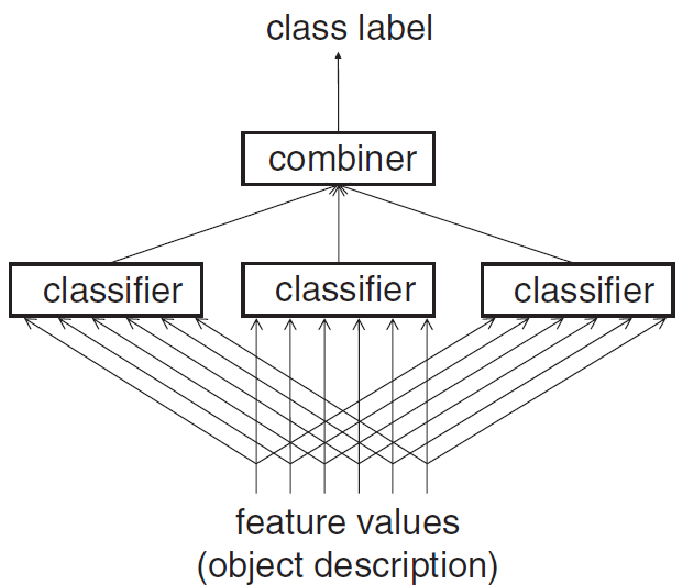
\includegraphics[width=.7\textwidth]{2_Background/figures/fig_ensemble-top.pdf}
 %   \caption{The simple topology for combining classifiers, taken from \cite{kuncheva2014}.}
  %  \label{ch2:ensemble-topology}
%\end{figure}










Each learning algorithm, Section \ref{sec:2_2_SML}, has a limit to discovering the hidden pattern. According to Wolpert's \emph{no free lunch} theorem \citep{wolpert2002}, there is no best classifier suitable for all problems, but each model has its own area of competence giving the design assumptions. For that, a set of learning models solving the same problem can be consolidated to generate a better composite global model \cite{ksieniewicz2018}. L. Kuncheva \cite{kuncheva2014} stated \textit{"the improvement of the ensemble over the single best classifier or even on the average of individual classifier accuracies is not guaranteed"}. From our perspective, the proper design of ensemble is conditioned by outperformance over the best individual classifier in the group.  



\subsection{Are we pursuing complexity?}
Why we accept complex systems instead of depending on a single classification algorithm?. The answer to this question is highlighted in the following points.
\begin{itemize}[nosep]
    \item[-] Ensemble models are the solution to deal with uncertainty. A solution from a single classifier can be boosted and trusted by aggregating a group of predictors (\textit{wisdom of crowds} \cite{rokach2010}).
    \item[-] There is no guide to design universal approximators, perfect model, i.e. it is difficult to set up ANNs or reaching their optimistic parameters.

    \item[-] Ensemble selection or pruning is an interesting research topic that aims to reduce ensemble complexity without deterioration in the performance.
\end{itemize}

In addition, a promising solution via ensemble learning can be achieved for the following scenarios:

\begin{itemize}[nosep]
    \item Imperfect Learning: Non-deterministic classifier can be considered as a local optimizer in terms of the training error, a safer option is to group several models that cover the solution space properly.
    \item Too much data: We are surrounded by too much data. In this case, data is split into chunks where similar or different learning algorithms can be trained on each part independently. Ensemble learning support parallelization and distributed computing for handling this scenario efficiently.
    \item Small-size data: In data shortage, stratified sampling with replacement can be applied, where several data replications will be obtained to train individual classifiers inside the ensemble. 
    \item Data fusion: The data pattern can be identified differently based on the data source. The availability of sensors strengthens decision making by analyzing different features. Instead of fusing all features and building a single classifier, it could be better to build a single classifier for each feature space and combine their decisions.  
    \item Complex hypothesis: Complex classification boundary can be approximated by combining several base classifiers.
    
\end{itemize}


\subsection{A Taxonomy of Classifier Ensemble Methods } \label{ch2.taxonomy}

A comprehensive review of the classifier ensemble methods, thorough discussion, and the development of further knowledge in this area was the core of many articles \cite{gonzalez2020,polikar2006,cruz2018, britto2014,re2012,sewell2008}, with a proposed taxonomy by L. Rokach \cite{rokach2009} who indicated the five dimensions to design this kind of powerful models. Figure \ref{ch2:ensemble-taxonomy} shows our perspective for the Multiple Classifier System (MCS) taxonomy as it has been proposed by L. Kuncheva \cite{kuncheva2014}, R. Cruz et al. \cite{cruz2018}, and L. Rokach \cite{rokach2009}. The two main phases in classifier ensembles are; Generation and Integration, while the selection is an intermediate/optional phase.   

\begin{figure}[!ht]
    \centering
    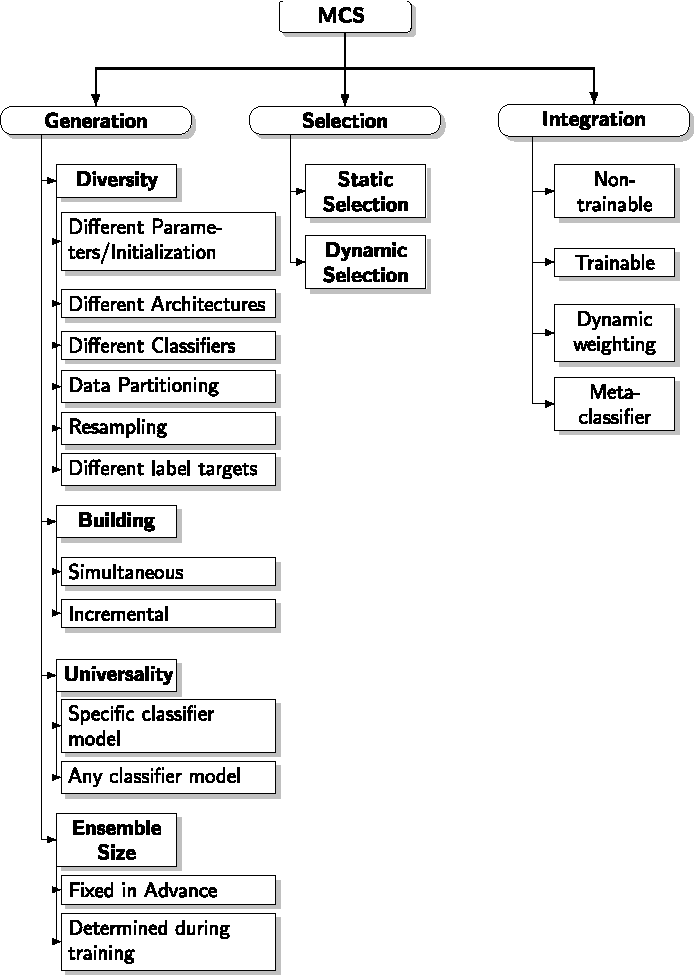
\includegraphics[width=.95\textwidth]{2_Background/figures/fig-taxonomy.pdf}
    \caption{The Taxonomy of Multiple Classifier System (MCS).}
    \label{ch2:ensemble-taxonomy}
\end{figure}



\subsubsection{Generation} \label{sub.generation}
The goal in this phase is to generate a pool of classifiers that are both diverse and accurate. This phase discusses strategies to handle data horizontally/vertically. In addition, what classifier type to accommodate, how to build the classifiers: dependent/independent manner, and how many classifiers to train (ensemble pool size). 

 \textbf{1) Diversity:}
Diversity is one of the main reasons for the effectiveness of ensemble methods \cite{zhou2012,gonzalez2020}. Diversified classifiers cause uncorrelated errors, which lead to improved classification accuracy \cite{hu2001}. In general, this can be achieved through the following six wide subcategories to promote diversity during the generation phase.
\begin{itemize}
    \item[-] \textbf{Different Parameters/Initialization:} \textit{Algorithm-level diversity}; via different parameters, the base classifiers can be generated by modifying the hyper-parameters of the learning algorithm; for example, controlling the number of $k$ neighbors, distance function in KNN model, and controlling the confidence level parameter in the decision tree. While, via different initialization and if the training process is initialization dependent, the model will be sensitive. In neural networks, different initial configurations of weights result in different decisions \cite{hansen1990}.        
  \item[-] \textbf{Different Architectures:}  \textit{Algorithm-level diversity}; this strategy is more suitable to multi-layer perceptron neural networks, where the number of hidden layers, the number of neurons, and the network topology affect the classifier domain space. For example; in the Addemup algorithm \cite{opitz1996}, the genetic algorithm is used to choose the required network topology to compose the ensemble according to a measure of diversity.     
  \item[-]\textbf{Different Classifier types:} \textit{Algorithm-level diversity}; each classifier model build its inference with a capability to discover a hidden pattern differently. Each model, Section \ref{sec:2_2_SML}, contains explicit or implicit bias that leads to a better generalization accuracy through combination. In addition, as in \cite {woods1997}, the divide and conquer mechanism is best implemented by calculating the local accuracy in the feature space to choose between four different classifier types.  
  \item[-]\textbf{Data Partitioning:} \textit{Data-level diversity}; Partitioning means the division into smaller disjoint components of the initial training. A different classifier will be trained on each part to gain different and accurate decision \cite{maimon2005}. This mechanism enables data mining algorithms to handle massive datasets by managing memory size and computational resources perfectly. The data can be partitioned horizontally or vertically. \textit{In horizontal partitioning}, several parts will be formed; each part will contain sub-samples while sharing the complete feature set. Sub-samples can reflect the entire dataset by selecting the instances from all the formed clusters of the dataset; known as cluster-based concurrent decomposition (CBCD) \cite{rokach2005}. The mixture of experts (ME) \cite{nowlan1991}   splits the input space into several subspaces and assign an expert, classifier, to each subspace. In \cite{cohen2007} a decision tree framework is employed to divide the input space into mutual exclusive partitions, then a new unseen pattern will be classified by a dedicated classifier that is learned from the space to which the instance belongs. \textit{In vertical partitioning}, The feature space is partitioned into several subsets keeping the same number of samples, then each classifier can be trained on a different projection. This mechanism is more suitable for a high-dimensional dataset without affection by the feature selection drawbacks \cite{tumer2003}, and the accuracy could be improved by the less correlation among classifiers. This division results in a high-speed classification algorithm \cite{bryll2003}, and solves the problem of class under-representation that exist with instance-based sampling.      
  
  \item[-]\textbf{Resampling:} \textit{Data-level diversity}; the diversity could be promoted by manipulating the training set. Each base model is trained over a different sample from the training. Bagging \cite{breiman1996,skurichina1998} and Boosting \cite{freund1997,freund1999} are the popular strategies in that paradigm. Bagging ensembles achieve a reasonable diversity level by creating different bootstrap samples to train each base model independently, then the final decision is adopted by a simple majority voting-based aggregation. Moreover, the non-sensitivity of bagging and robustness under diverse noise conditions makes it more attractive \cite{dietterich2000}. Contrary to sequential ensembles, \textit{Boosting}, the individual members are generated in the sequential schema by the learning algorithm \cite{freund1997}. The sequential mechanism of boosting encourages the complementariness between ensemble members, by focusing on previously misclassified samples. However, the performance in boosting is more sensitive to noisy samples \cite{dietterich2000,caruana2006} and sometimes overfitting can be observed for large pool size \cite{ratsch2001}. 
  
  \item[-]\textbf{Differnet label targets:} \textit{Data-level diversity}; manipulating the target attribute is very interesting mechanism to promote diversity. Instead of building complex classifier, several classifiers with usually simpler representations, about the target attribute, will be trained. For instance, to handle the multi-class dataset, the original target attribute can be replaced by a simpler and smaller target domain. Among those strategies, One versus all (OVA) \cite{anand1995} which divides the $M$-class classification problem into $M$ two-class classification tasks. While one versus one (OVO) \cite{lu1999} divides the $M$-class classification problem into $M(M-1)/2$ two-class classification tasks, so the complex decision boundary can be simplified. Minimal classification method (MCM) \cite{sivalingam2005} converts the $M$-class classification task to the minimal binary classification tasks. MCM requires $\log_2(M)$ classification tasks in the form of a separation between groups of multiple classes. Furthermore, the error-correcting output coding (ECOC) algorithm, uses a code matrix to decompose the multiclass problem into multiple binary problems \cite{dietterich1994}. In addition, label switching algorithms \cite{breiman2000,martinez2005} change the labels of samples picked randomly. 
\end{itemize}


\textbf{2) Building:}
This part discusses the building schema to generate a pool of classifiers, whether to be dependent or independent. In the dependent framework (sequential/incremental), the performance of a classifier affects the creation of the next classifier in the chain. Instead, in the independent framework (simultaneous), the classifiers are generated independently. 

\begin{itemize}
    \item[-]\textbf{Simultaneous:} The independent methods to generate a set of classifiers mainly depends on forming different training samples from the original training set. The training samples could be mutually exclusive (disjointed) or overlapping. The reason behind preferring this schema is to improve the predictive accuracy or to speed up the generation step as this schema supports parallel implementation. \textit{Bagging} (Bootstrap AGGregatING) \cite{breiman1996} is the popular method in this category, with a replacement from the original training set, each classifier is trained on data samples. The sample size will be equivalent to the original training size; randomly some samples will be duplicated and some samples will be ignored.  
     \item[-]\textbf{Incremental:} Sometimes called dependent, there is a kind of interconnection during the learning process. The model generation depends on the accuracy of the previous model/committee. The training process is done in iterative form, where the learning process will be directed to focus on the previously misclassified samples. \textit{Boosting} \cite{freund1996} (also known as arcing- Adaptive Resampling and Combining) is the popular method in this category. The training process mainly depends on assigning weights to all the training samples. In the beginning, all the samples will be equally weighted (having the same importance), but throughout the iterations, the weights of correctly classified samples are lowered while the weights of misclassified samples are raised. As a consequence, the base model is directed to focus on the hard samples in the training set.          
\end{itemize}


\textbf{3) Universality:}
This part discusses the universality of the ensemble model. Some ensembles techniques could be designed to work for any classifier, while other ensembles have been designed to work with specific classifiers. In other meaning, the relation between the ensemble technique and the used classifier type. 

\begin{itemize}
    \item[-]\textbf{Specific Inducer:} Known as inducer-dependent ensembles, where the effectiveness of the ensemble could be degraded if applied for other classifier types. For example, \cite{hansen1990,lu1999} those ensembles are explicitly designed for neural networks. Additional schemas \cite{tao2006} are perfectly suited for SVM.
    
     \item[-]\textbf{Any Inducer:} Known as inducer-independent ensembles, Those implementations can be extended to a wide variety of classifier types without affecting the generalization accuracy. 
    
\end{itemize}


\textbf{4) Ensemble Size:}
This part discusses the aspect of pool size. How many classifiers should be trained?. The main four factors that concern the ensemble size as determined by L. Rokach \cite{rokach2009} are; (A) \textit{Sufficient Accuracy}; the appropriate accuracy of the ensemble could be reached by aggregating 10 models \cite{hansen1990}, while other empirical studies show that this level of accuracy is correlated with large-size ensembles containing 25 models \cite{opitz1999}. (B) \textit{Computational Cost}; the more classifiers are generated the more computational resources are consumed. As a consequence, the user may predetermine the pool size to match the computational cost limits. (C) \textit{Nature of Task}; the ensemble size could be problem-dependent, as we stated before with the ensemble size of OVO and OVA strategies for handling multi-class classification tasks. (D) \textit{Number of processor cores}; for independent ensembles, the number of internal cores can be the upper bound to control how many classifiers can be trained in parallel mode.                      

\begin{itemize}
    \item[-]\textbf{Fixed in Advance:} This is the simple form to predetermine how many iterations should be considered. Most Bagging and Boosting software packages give the flexibility to control the number of iterations.  
    
     \item[-]\textbf{Determined during Training:} The best ensemble size can be determined during train time. The contribution of a new classifier to the ensemble performance is to be checked if it is significant or not. To estimate the unbiased error of the test sample, Random Forests uses the out-of-bag (OOB) procedure. The OOB error estimation is used in \cite{banfield2006} to determine the sufficient number of classifiers. As the maximum accuracy no longer increases, the training procedure stops.       
    
\end{itemize}



\subsubsection{Selection}
There is no value from combining similar classifiers' decisions. The effectiveness of the ensemble is conditioned by the diversity and the correctness of the base classifiers. Ensemble Selection is one of the strategies that can be used to handle this challenge. Ensemble Selection has been known in the literature as ensemble pruning \cite{lu2010,zhang2006,ykhlef2017}, ensemble thinning \cite{banfield2005} and ensemble reduction \cite{diao2013,zhang2018}. ES can be considered as an intermediate process between building the ensemble and aggregating the decisions. Specifically, ES is the strategy of optimizing and selecting the number and the type of individual classifiers in-advance. Collecting the decisions from a reduced number of models speeds up the classification systems and relieves memory storage. In the literature, the selection process can be performed offline, static selection \cite{tsoumakas2009}, or online, dynamic selection \cite{cruz2018}.
 
 
 \begin{itemize}
    \item[-]\textbf{Static Ensemble Selection:} Known in the literature review as ensemble pruning. This process is done during the training and before the real test. A subset of classifiers that optimize a predefined function/metric are selected, and the estimation of that metric is done over a pruning set. The most common metrics/selection criteria are; diversity \cite{aksela2003,brown2010}, classification accuracy \cite{dos2009,ruta2005}, instance margin \cite{yang2012, guo2013,hernandez2008}. However, it is not trivial to find the optimal subset of classifiers from a large ensemble as the complexity increases exponentially with the pool size. Researchers agreed in common that ES is a combinatorial search problem with $2^{T}-1$ nonempty subsets to be evaluated from pool size, $T$, to find the best subset \cite{tamon2000, tsoumakas2009}. To handle this complexity, several attempts ranging from optimized search \cite{diao2013,adnan2016,ruta2001b}, clustering techniques \cite{onan2017,zyblewski2020}, and greedy algorithms \cite{cao2018,martinez2009,margineantu1997, partalas2010, mao2011} have been applied over decades. More details about ordering-based pruning will be discussed in Section \ref{ch5_ordering_pruning}.        
    
     \item[-]\textbf{Dynamic Ensemble Selection:} This process is done during the test time. A single classifier or subset of classifiers are selected based on the unseen sample. In addition, dynamic weights are assigned according to the competition among individual classifiers over the local region of an unknown sample $\textbf{x}$. As a consequence, the selected subset is changeable for each test pattern \cite{KO2008}. This process consists of three steps; (1) Definition of the local region surrounding the query sample $\textbf{x}$, (2) Determination of the selection criteria to estimate the competence level of the classifiers, and (3) Determination of the selection mechanism, whether to select a single classifier or ensemble of classifiers. Without debate, dynamic selection techniques can outperform the static selection methods as experimentally been proved in \cite{cruz2018} since the selection is optimized for each test sample independently. The rationale in dynamic selection is that each classifier is an expert in a different local region within the feature space. However, in the dynamic selection, there is a computational overhead for selecting subensemble for each test sample. Besides, those techniques flood the memory space as all individual classifiers have to be retained in memory. Additionally, the dynamic selection is affected by the outlier instances around the query sample in the feature space \cite{CRUZ2015}.
    
\end{itemize}

Cluster and pick \cite{kuncheva2000} is a poor variant of dynamic selection. Initially, the input space is split into disjoint regions via clustering the training samples. The best classifier is then defined and chosen for each cluster. Cluster and select is in-between static and dynamic strategies; the classifiers are selected dynamically depending on which region the input sample belongs to, but the regions are static, determined in advance during the training \cite{ruta2005}.

 
 
 
\subsubsection{Integration}
Also known as the combiner function. The combiner balances the deviation between the diversity and the bias, also alleviates the errors that certain models have made \cite{SOARES2013}. This process concerns the methodology by which the outputs of the base classifiers will be aggregated.  A vital phase in building a group of classifiers is the use of a suitable fusion strategy to aggregate response decisions \cite{zhou2012,kuncheva2014}. The responses of individual classifiers restrict the fusion method and enhance or degrade the composite prediction. Those responses may be on the \textit{abstract level} \cite{xu1992}, where each classifier specifies a class name as a decision. Additionally, the responses may be \textit{ranked levels} \cite{PARKER2001}, where each classifier outputs a ranked subset of class labels, or even  \textit{measurement values} \cite{kuncheva2014a,niu2007}, where each classifier specifies a posterior probability.


\begin{itemize}
    \item[-]\textbf{Non-trainable:} 
    The combination function does not require any training from the classifiers' decision space. Many combination rules have been proposed; for measurement values (Sum, Product, Maximum, Minimum, Median, and Decision Templates \cite{Kuncheva2001}), for abstract level (Majority voting \cite{Kittler1998}, Behavior Knowledge Space \cite{Huang1995}, and Naive Bayes \cite{xu1992}), and for ranked levels (Borda count \cite{Ho1994}). The majority voting, Equation(\ref{majority}), will be effective if the base classifiers are independent. While, the weighted sum rule, Equation(\ref{weighted.sum}), produces good results if the classifiers perform the same task and have comparable success or when we would like to avoid over-fitting or long training time \cite{rokach2009}. The weights, $w_k$, are calculated to be proportional to the individuals' performance over a validation dataset.  In addition, weighted voting is preferred for highly imbalanced datasets \cite{kuncheva2014a,krawczyk2014}.  
    
\begin{equation}
\label{majority}
\hat{\Psi}(\textbf{x})=\mathop{\arg\max}\limits_{c \in \mathcal{M}} \mathop{\sum}\limits_{k=1}^T \left[\Psi_k(\textbf{x})=c\right] 
\end{equation}    

\begin{equation}
\label{weighted.sum}
\hat{\Psi}(\textbf{x})=\mathop{\arg\max}\limits_{c \in \mathcal{M}} \mathop{\sum}\limits_{k=1}^T \left[\Psi_k(\textbf{x})=c\right]w_k
\end{equation}
    
    
     \item[-]\textbf{Trainable:}  
The combination function is to be configured specifically to the classification task. The aggregation function will be trained over a validation dataset from the domain, \textit{base classifiers outputs}, and co-domain, \textit{real attribute output}. For example; the classifiers' fusion weights can be optimized by evolutionary algorithms (EA).  In \cite{krawczyk2014}, the authors tuned the weights for the selection and fusion of multiple cost-sensitive decision trees to handle imbalanced data using the evolutionary genetic algorithm (GA) \cite{mitchell1998}. Each chromosome from the genetic population simulates a weighted ensemble as $\left[w_1, w_2, \ldots, w_k, \ldots w_T\right]^T$, $ \forall w_k \in [0,1]$. The ensemble performance is estimated for each chromosome, and genetic operators evolve the next generations. In addition, GA has been applied in \cite{sikora2015} to tune the weights of heterogeneous classifiers in consideration of the above chromosome encoding. While, a bird-flock based optimization algorithm has been applied in \cite{cordeiro2011, kausar2010} to enhance the fusion process.          
      
\item[-]\textbf{Meta-classifier:}   
Meta-learner is another important fusion mechanism. It is a trainable method, where the aggregation function is to be learned based on the base classifiers outputs. \textit{Stacking} \cite{Wolpert1992} is the most popular meta-learning method, where the predictions from the base classifiers become meta-features/inputs to a new classifier. The original target attribute from the training set remains as it is. Stacking
is generally used to combine heterogeneous models, the term refers to stacking layers of classifiers. In stacking, the correctness of the base classifiers will be learned indirectly through the meat-learner. In \textit{Grading} \cite{seewald2001}, the predictions of base classifiers are transformed into true or false. After that, one meta-classifier will be trained on the transformed decisions of one base model to learn when it errors. Therefore, grading can be seen as a generalization of cross-validation selection, by using only those classifiers that correctly predict specific instances. 



\item[-]\textbf{Dynamic weighting:} Similar to dynamic ensemble selection. The classifiers' fusion weights are determined dynamically based on the local competence of the classifier in the region where the unknown $\textbf{x}$ is located. A higher weight value is assigned to the most competent classifier  \cite{cruz2018}. For example, dynamic integration of classifiers in \cite{Tsymbal2008}. In addition, the dynamic ensemble selection and the dynamic ensemble weighting can be hybrid as in \cite{KO2008}.       
\end{itemize}


Finally, Figure \ref{ch2:four-levels} shows the questions that should be answered during the four levels of constructing MCS \cite{kuncheva2014}.     

\begin{figure}[!ht]
    \centering
    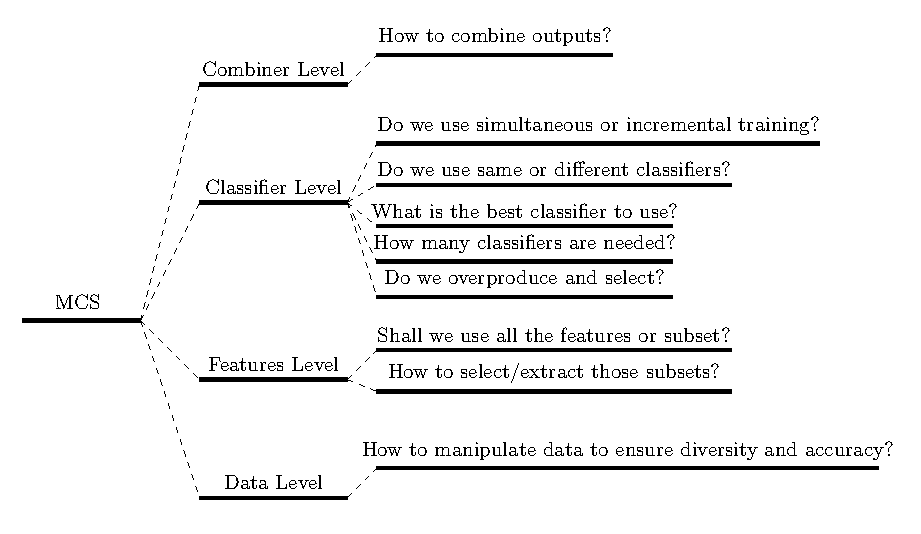
\includegraphics[width=\textwidth]{2_Background/figures/fig-four-levels.pdf}
    \caption{ Four level questions while building MCS.}
    \label{ch2:four-levels}
\end{figure}


\subsection{Diversity and Uncorrelated Errors}
Indeed the two basic facets of enhancing the efficacy of the committee are often referred to as decision optimization and coverage optimization \cite{ho2002}. \textit{Decision optimization} refers to methods for choosing and optimizing the combination method. \textit{Coverage optimization} refers to the techniques used to construct a diverse classifier set, assuming a fixed combiner. In Section \ref{sub.generation}, the prospective methods to generate diverse base models were reviewed. 
If a classifier makes errors on some objects, then it is better to complement it with another classifier that compensates that error. The ensemble performance is restricted by a compromise between an individual's accuracy and group diversity. Confirmed as, neither the individual's accuracy \cite{rogova1994} nor the diversity \cite{ruta2001a} on their own provide reliable ensemble to outperform the best individual classifier. Here, we agree with  L. Kuncheva \cite{kuncheva2014}, ''\textit{good estimate can be obtained from arbitrarily inaccurate estimators as long as their deviations cancel one another}''. However, it is so difficult to engineer this ensemble design.   


There is no benefit from combining redundant classifiers, and the system will be more complex. A large number of classifiers increase the ambiguity, risk, and add more complexity to the selection procedure which could lead to weak generalization \cite{ruta2005}. While for critical systems the useful evidence is so important and should not be wasted. Regarding that, more attempts have been made to select classifiers based on diversity measures. In \cite{giacinto2001}, the authors used a double fault measure to cluster classifier outputs, then they picked a single classifier from each cluster. While in \cite{kim1997} a similarity measure is used to pick a classifier from a pool of five classifiers. Many diversity measures have been presented \cite{kuncheva2003,ruta2001a} with the conclusion that diversity guided search could be invaluable. In addition, the diversity has been intensively used with the combiner performance \cite{ruta2005,li2012,brown2010} to improve the efficiency. The system design does not end with the selection process, as the selected classifiers should be next combined. For that, there should be a correlation between diversity measure value and committee performance. Diversity initiatives that represent at least some clear association trends, with generalization, have the potential to become appropriate criteria for selection. Diversity measurement is not a trivial task in ensemble methods. 


Matti et.al \cite{aksela2006} stated that diversity can be measured from two perspectives, Figure \ref{ch2:diversity-measures}, based on the population. (a) \textit{The data-based approach:} we have $N$ populations with $T$ objects. The ensemble diversity of the $T$ classifiers is calculated for each sample $\textbf{x}_i$, then the overall average is considered over $N$ samples. Here the diversity of all member classifiers is evaluated simultaneously (Non-Pairwise measurement). (b) \textit{The classifier-based approach:} in this case we have $T$ populations each contain $N$ objects. The diversity is to be calculated based on the classifiers' outputs for all input data. Each pair of classifiers are considered for measuring the diversity, then the overall diversity is computed by averaging over the number of pairs (Pairwise measurement).       

\begin{figure}[!ht]
    \centering
    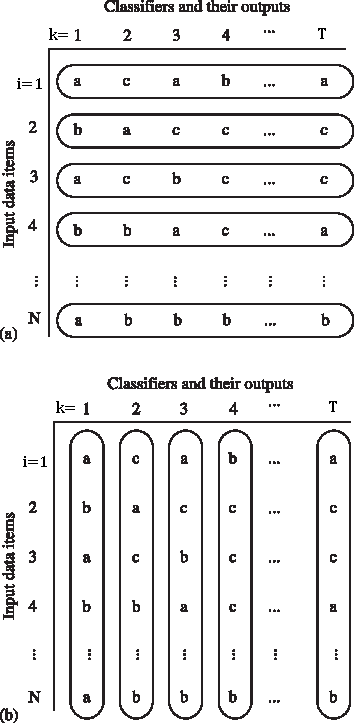
\includegraphics[width=.5\textwidth]{2_Background/figures/fig-diveristy-measure.pdf}
    \caption{Diversity measure approaches for MCS: (a) data-based, and (b) classifier-based, taken from \cite{aksela2006}.}
    \label{ch2:diversity-measures}
\end{figure}




Next, a set of popular measures are presented based on the correct/incorrect outputs. First, the output of $\Psi_k$ can be represented as N-dimensional binary vector $y_k= \left[y_{1k}, y_{2k}, \ldots, y_{Nk}\right]^T$, such that $y_{ik}$=1, if $\Psi_k$ recognizes $\textbf{x}_i$ correctly, and 0 otherwise, $k=1,2,\dots,T$. Moreover, the relationship between a pair of classifiers ( $\Psi_j$, $\Psi_{k}$ ) can be represented as in Table \ref{classifier.relation}. 

  \begin{table}[!ht]
 \centering \scriptsize
 \caption{2 $\times$ 2 table of the relationship between a pair of classifiers.}
\label{classifier.relation}
\begin{tabular}{l|cc}
\hline
 & $\Psi_k$ correct (1) & $\Psi_k$ wrong (0)  .\\ \hline

$\Psi_{j}$ correct (1)  & $N^{11}$ & $N^{10}$  \\
$\Psi_{j}$ wrong (0)  & $N^{01}$& $N^{00}$ \\ \hline
\multicolumn{2}{c}{Total, $N=N^{00} + N^{01} + N^{10}+ N^{11} $} & \\

\hline
\end{tabular}
\end{table}   


\subsubsection{Pairwise diversity measures}

\begin{enumerate}
    \item \textit{The Q statistics :} Is a various statistic measure to measure the similarity of two classifier outputs. The \textit{Q} statistics for two classifiers, $\Psi_j$ and $\Psi_{k}$ is: 

\begin{equation}
\label{Q.statistics}
 Q_{j,k}=\frac{N^{11}N^{00}-N^{01}N^{10}}{N^{11}N^{00}+N^{01}N^{10}}
\end{equation}

Symbols are explained in Table \ref{classifier.relation}. \textit{Q} varies between -1 and 1. Classifiers that agree on the same objects will have positive \textit{Q} values, and those that make mistakes on different objects will have negative \textit{Q} values. The averaged statics over all pairs of classifiers is:


\begin{equation}
\label{averaged.qstatistics}
Q_{avg}=\frac{2}{T(T-1)} \mathop{\sum}\limits_{j=1}^{T-1} \mathop{\sum}\limits_{k=j+1}^T Q_{j,k}   \end{equation}
    
 \item \textit{The correlation coefficient 	$\rho$ :}  
 The correlation between two binary classifier outputs can be calculated as:   
   

\begin{equation}
\label{correlation.cofficient}
 \rho_{j,k}=\frac{N^{11}N^{00}-N^{01}N^{10}}{\sqrt{(N^{11} + N^{10})(N^{01} + N^{00})(N^{11} + N^{01})(N^{10} + N^{00})}}
\end{equation}    
    
For any two classifiers, $Q$ and $\rho$ have the same sign, and it can be proved that $|\rho|$ $\le |Q|$. 
  
  
\item \textit{The disagreement measure :}    
This measure has been used by HO \cite{ho1998} to measure the diversity in decision forests. It is the ratio between the number of samples on which one classifier disagree with another, to the total number of samples.

\begin{equation}
\label{disagreement.metr}
 Dis_{j,k}=\frac{N^{01} + N^{10}}{N^{11}+ N^{10}+N^{01}+N^{00}}
\end{equation}  
    
    
\item \textit{The double-fault measure :}     
It is defined as the proportion of samples on which both classifiers makes error, i.e.,

\begin{equation}
\label{default.measure}
 DF_{j,k}=\frac{N^{00}}{N^{11}+ N^{10}+N^{01}+N^{00}}
\end{equation}  

    
For all pairwise measures, the averaged values are calculated similarly to Equation (\ref{averaged.qstatistics}).       
\end{enumerate}
 
 
 
 
\subsubsection{Non-Pairwise diversity measures}

\begin{enumerate}
   
 \item \textit{The entropy measure E :}    The highest diversity among classifiers for a particular $\textbf{x}_i \in \textbf{X}$ is proved by $\floor{T/2}$ of the votes for $\textbf{x}_i$ with the same value (0 or 1) and the other $T - \floor{T/2}$ with the alternative value. If all decisions are 0's or all are 1's, then there is no diverse. Denote by $t(\textbf{x}_i$) the number of classifiers that correctly classify $\textbf{x}_i$, i.e,  $t(\textbf{x}_i$)=$\sum_{k=1}^{T} \Psi_{ik}$. On the basis of this concept, the diversity can be measured as:
    
   \begin{equation}
\label{Entropy.measure}
 E=\frac{1}{N} \sum_{i=1}^{N} \frac{1}{(T-\ceil{T/2})} \text{min}\{t(\textbf{x}_i),T-t(\textbf{x}_i)\}
\end{equation}   
  
$E$ ranges between 0 and 1, where 0 implies no difference, whereas high diversity is measured by 1.  
  
\item \textit{Kohavi-Wolpert variance :} It measures the average variance between the binomial distributions of the outputs of each classifier. This measure can be simply calculated by :
 
   \begin{equation}
\label{Kohavi.measure}
 KW=\frac{1}{NT^2} \sum_{i=1}^{N} t(\textbf{x}_i)(T-t(\textbf{x}_i))
\end{equation}   
  
  
 \item \textit{Measurement of interrater agreement $\kappa$ :} It is used to measure the level of agreement while correcting the chance. let's denote $\Bar{p}$ as the average individual classification accuracy, i.e.,
 
\begin{equation}
\label{individual.accuracy}
 \Bar{p}=\frac{1}{NT} \sum_{i=1}^{N}\sum_{k=1}^{T} \Psi_{ik}
\end{equation}   
  
 
 then, the interrater agreement could be formulated as:
 
\begin{equation}
\label{interrater.agreement}
 \kappa=1-\frac{\sum_{i=1}^{N}t(\textbf{x}_i)(T-t(\textbf{x}_i))}{NT(T-1)\Bar{p}(1-\Bar{p})} 
\end{equation} 
    
\end{enumerate}





 
\subsubsection{Uncorrelated Errors } \label{ch2_uncorrelated}

Standard diversity measures do not take into account that for classification purposes, identical correct decisions are preferred over identical erroneous decisions. It may be useful to analyze, in particular, the errors made by committee members. In this case, we will focus on the error types and whether this error occurs or not by the base models. If two classifiers incorrectly classify a sample into two separate categories, then this case is known as \textit{uncorrelated errors/diversity of errors}, as the predicted class is not the same despite the fact that both make mistake. The most difficult samples are the cases where all classifiers agree to the same incorrect class. Diversity measures that capture the type of error are initiatives and powerful as they can solve the following challenges:


    


\begin{itemize}[nosep]
\item[-] There are a few correct recognition results in most recognition tasks, while it is hard for the combination function to predict the correct output from this whole set of incorrect predictions. This can be solved by knowing the class of error.
\item[-] Classifiers that agree on the correct outcome should be credited rather than eliminated when selecting classifiers, however, this is conflicting with the principle of diversity maximization. 
\end{itemize}
 
\noindent Naturally, It is best if all classifiers make a correct prediction and it is better if we have fewer classifiers make a mistake. Even, for those mistakes, it is exceedingly helpful if the errors are different as often as possible, i.e. maximum diverse errors. Hence, the oracle-level (binary) classifier outputs should be interconnected with the predicted class category to identify the diversity of errors.


As stated in the introduction of this part, the difference in the mistakes made by the member classifiers really affects the performance. Given the following notations; $N_{same}^{00}$ indicates the number of samples when both classifiers are inaccurate and suggest the same decision. $N_{diff}^{00}$ stands for the number of samples when both classifiers are incorrect, but suggest different decisions. Next, let's present metrics \cite{aksela2006} that could be used to measure the diversity of errors: 

\begin{enumerate}
   
 \item \textit{Same-fault measure :} In an extension of the Double-Fault measure, the simultaneous fault could be restricted to measure when both classifiers are inaccurate  and suggest the same output. This can be measured for two classifiers $\Psi_j$ and $\Psi_{k}$ as:
 
 
 \begin{equation}
\label{samefault.measure}
 SF_{j,k}=\frac{N_{same}^{00}}{N^{11}+ N^{10}+N^{01}+N^{00}}
\end{equation}  
 
Then the averaged pairwise measures could be calculated similarly to Equation (\ref{averaged.qstatistics}). The optimal classifier set is picked based on the minimum measure.


\item \textit{Weighted count of errors and correct results:} It is designed to consider information about correct prediction. The number of samples that match specific cases can be weighted; based on classifier outputs, "both correct" is favorable and classifiers of this type are highly selected via increasing the weights. While "both incorrect and same" are highly penalized by assigning high negative weight, this can be defined for two classifiers $\Psi_j$ and $\Psi_{k}$ as: 
 
 
 \begin{equation}
\label{weighted.count.errors}
WCEC_{j,k}=N^{11}+\frac{1}{2}(N^{10}+N^{01}) -N_{diff}^{00}-5N_{same}^{00}
\end{equation}   
 
Moreover, based on the combiner's performance over the training set, the weights above could be optimized. The averaged pairwise measures are calculated similarly to Equation (\ref{averaged.qstatistics}), and the optimal classifier set is picked based on the maximum measure.  

\item \textit{Exponential error count :} As more errors are encountered the classifier capability will be hindered. Here, this concept is emphasized by counting the number of errors and assigning a weight in an exponential fashion. Assume $\Psi_{same}^{k \times 0}$ denote the number of errors made by $k$ classifiers to the same class, then the measure can be defined as:

\begin{equation}
\label{exponential.error.count}
EEC_{(\Psi_1,\dots,\Psi_T)}= \frac{\sum_{k=1}^{T} (\Psi_{same}^{k \times 0})^k }{N^{T \times 1}+1}
\end{equation} 
 
This measure considers all classifiers set. In addition, the correct classification is considered by scaling the exponential sum with $N^{T \times 1}$ (the number of samples for which every member classifier was correct). The optimal classifier set is picked based on the minimum measure.    
 
 \end{enumerate}





